\section*{Introduction}

\begin{frame}{Introduction}
    \begin{itemize}
        \item Single-agent shortest path planning: given a graph, compute a path from a start node $s$ to a goal $t$ whose cost is minimum;
        \item Modern algorithms use auxiliary data structures to improve performances;
        \item However, when \textbf{edge costs are dynamic} such algorithms may fail due to invalid auxiliary data.

        \item \textbf{Goal}: Solve dynamic-cost single agent path planning problems by exploiting Compressed Path Database (CPD);
        \item \textbf{Results}: new bounded A* variant using CPD whose experimentally-evaluated performances show substantial gains over previous algorithms.
    \end{itemize}
\end{frame}

% see https://tex.stackexchange.com/a/208409/145331
\begin{frame}[fragile]{A simple example}

    \only<1>{
        \begin{center}
            \textbf{Original Map}

            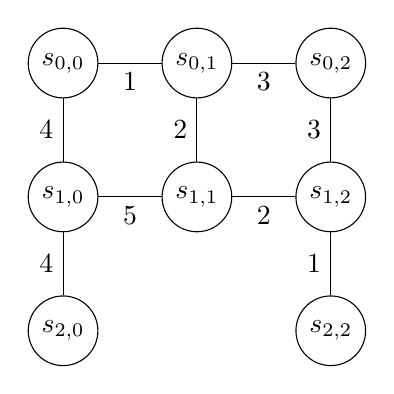
\begin{tikzpicture}
                \tikzset{Vertex/.style={%
                    shape=circle,%
                    draw=black,%
                    minimum size=10pt,%
                    radius=1cm,%
                    inner sep=3pt,%
                    node distance=1.7cm,%
                }}
        
                \node[Vertex] (v00) at (0,0) {$s_{0,0}$};
                \node[Vertex, right of=v00] (v01) {$s_{0,1}$};
                \node[Vertex, right of=v01] (v02) {$s_{0,2}$};
                \node[Vertex, below of=v00] (v10) {$s_{1,0}$};
                \node[Vertex, right of=v10] (v11) {$s_{1,1}$};
                \node[Vertex, right of=v11] (v12) {$s_{1,2}$};
                \node[Vertex, below of=v10] (v20) {$s_{2,0}$};
                \node[Vertex, below of=v12] (v22) {$s_{2,2}$};
        
                \path (v00) edge[-.] node[below]{1} (v01);
                \path (v01) edge[-.] node[below]{3} (v02);
                \path (v10) edge[-.] node[below]{5} (v11);
                \path (v11) edge[-.] node[below]{2} (v12);
                \path (v00) edge[-.] node[left]{4} (v10);
                \path (v10) edge[-.] node[left]{4} (v20);
                \path (v01) edge[-.] node[left]{2} (v11);
                \path (v02) edge[-.] node[left]{3} (v12);
                \path (v12) edge[-.] node[left]{1} (v22);
            \end{tikzpicture}
        \end{center}
    }%
    \only<2>{
        \begin{center}
            \textbf{Original Map}

            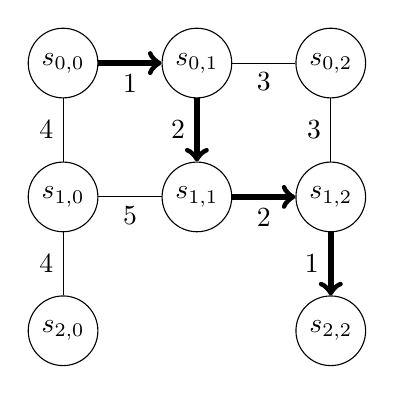
\begin{tikzpicture}
                \tikzset{Vertex/.style={%
                    shape=circle,%
                    draw=black,%
                    minimum size=10pt,%
                    radius=1cm,%
                    inner sep=3pt,%
                    node distance=1.7cm,%
                }}
        
                \node[Vertex] (v00) at (0,0) {$s_{0,0}$};
                \node[Vertex, right of=v00] (v01) {$s_{0,1}$};
                \node[Vertex, right of=v01] (v02) {$s_{0,2}$};
                \node[Vertex, below of=v00] (v10) {$s_{1,0}$};
                \node[Vertex, right of=v10] (v11) {$s_{1,1}$};
                \node[Vertex, right of=v11] (v12) {$s_{1,2}$};
                \node[Vertex, below of=v10] (v20) {$s_{2,0}$};
                \node[Vertex, below of=v12] (v22) {$s_{2,2}$};
        
                \path (v00) edge[->,line width=2pt] node[below]{1} (v01);
                \path (v01) edge[-.] node[below]{3} (v02);
                \path (v10) edge[-.] node[below]{5} (v11);
                \path (v11) edge[->,line width=2pt] node[below]{2} (v12);
                \path (v00) edge[-.] node[left]{4} (v10);
                \path (v10) edge[-.] node[left]{4} (v20);
                \path (v01) edge[->,line width=2pt] node[left]{2} (v11);
                \path (v02) edge[-.] node[left]{3} (v12);
                \path (v12) edge[->,line width=2pt] node[left]{1} (v22);
            \end{tikzpicture}

            $$s_{0,0} \rightarrow s_{0,1} \rightarrow s_{1,1} \rightarrow s_{1,2} \rightarrow s_{2,2}$$
        \end{center}
    }%
    \only<3>{
        \begin{center}
            \textbf{Perturbated Map}

            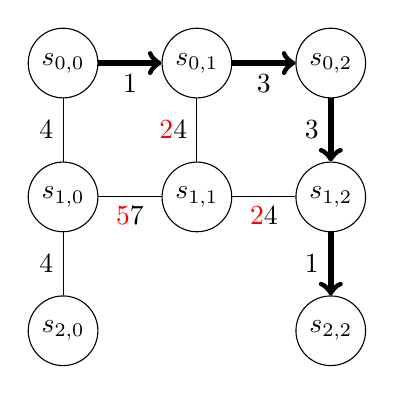
\begin{tikzpicture}
                \tikzset{Vertex/.style={%
                    shape=circle,%
                    draw=black,%
                    minimum size=10pt,%
                    radius=1cm,%
                    inner sep=3pt,%
                    node distance=1.7cm,%
                }}
        
                \node[Vertex] (v00) at (0,0) {$s_{0,0}$};
                \node[Vertex, right of=v00] (v01) {$s_{0,1}$};
                \node[Vertex, right of=v01] (v02) {$s_{0,2}$};
                \node[Vertex, below of=v00] (v10) {$s_{1,0}$};
                \node[Vertex, right of=v10] (v11) {$s_{1,1}$};
                \node[Vertex, right of=v11] (v12) {$s_{1,2}$};
                \node[Vertex, below of=v10] (v20) {$s_{2,0}$};
                \node[Vertex, below of=v12] (v22) {$s_{2,2}$};
        
                \path (v00) edge[->,line width=2pt] node[below]{1} (v01);
                \path (v01) edge[->,line width=2pt] node[below]{3} (v02);
                \path (v10) edge[-.] node[below]{{\color{red} \xcancel{5}}{7}} (v11);
                \path (v11) edge[-.] node[below]{{\color{red} \xcancel{2}}{4}} (v12);
                \path (v00) edge[-.] node[left]{4} (v10);
                \path (v10) edge[-.] node[left]{4} (v20);
                \path (v01) edge[-.] node[left]{{\color{red} \xcancel{2}}{4}} (v11);
                \path (v02) edge[->,line width=2pt] node[left]{3} (v12);
                \path (v12) edge[->,line width=2pt] node[left]{1} (v22);
            \end{tikzpicture}

            $$s_{0,0} \rightarrow s_{0,1} \rightarrow s_{0,2} \rightarrow s_{1,2} \rightarrow s_{2,2}$$
        \end{center}
    }
    
\end{frame}


% \begin{frame}[fragile]{A simple example}
%     \begin{center}
%         \textbf{Original Map}\\
%     \end{center}

%     \begin{minipage}{0.5\textwidth}
%         \begin{tikzpicture}
%             \matrix[square matrix]{
%                 |[fill=black!0]| $s_{0,0}$   &|[fill=black!0]| $s_{0,1}$  &|[fill=black!40]| $s_{0,2}$  \\
%                 |[fill=black!60]| $s_{1,0}$   &|[fill=black!20]| $s_{1,1}$  &|[fill=black!0]| $s_{1,2}$  \\
%                 |[fill=black!0]| $s_{2,0}$   &|[fill=black]|  &|[fill=black!0]| $s_{2,2}$  \\
%             };
%         \end{tikzpicture}
        
%         \begin{tabular}{clcl}
%             \drawFilledSquare{black!0} & 1 &
%             \drawFilledSquare{black!20} & 3 \\
%             \drawFilledSquare{black!40} & 5 &
%             \drawFilledSquare{black!60} & 7 \\
%             \drawFilledSquare{black} & $\infty$ &
%             & \\
%         \end{tabular}
%     \end{minipage}%
%     \begin{minipage}{0.5\textwidth}
%         \begin{tikzpicture}
%             \tikzset{Vertex/.style={%
%                 shape=circle,%
%                 draw=black,%
%                 minimum size=10pt,%
%                 radius=1cm,%
%                 inner sep=3pt,%
%                 node distance=1.7cm,%
%             }}
    
%             \node[Vertex] (v00) at (0,0) {$s_{0,0}$};
%             \node[Vertex, right of=v00] (v01) {$s_{0,1}$};
%             \node[Vertex, right of=v01] (v02) {$s_{0,2}$};
%             \node[Vertex, below of=v00] (v10) {$s_{1,0}$};
%             \node[Vertex, right of=v10] (v11) {$s_{1,1}$};
%             \node[Vertex, right of=v11] (v12) {$s_{1,2}$};
%             \node[Vertex, below of=v10] (v20) {$s_{2,0}$};
%             \node[Vertex, below of=v12] (v22) {$s_{2,2}$};
    
%             \path (v00) edge[-.,line width=2pt] node[below]{1} (v01);
%             \path (v01) edge[-.] node[below]{3} (v02);
%             \path (v10) edge[-.] node[below]{5} (v11);
%             \path (v11) edge[-.,line width=2pt] node[below]{2} (v12);
%             \path (v00) edge[-.] node[left]{4} (v10);
%             \path (v10) edge[-.] node[left]{4} (v20);
%             \path (v01) edge[-.,line width=2pt] node[left]{2} (v11);
%             \path (v02) edge[-.] node[left]{3} (v12);
%             \path (v12) edge[-.,line width=2pt] node[left]{1} (v22);
%         \end{tikzpicture}
%         $$s_{0,0} \rightarrow s_{0,1} \rightarrow s_{1,1} \rightarrow s_{1,2} \rightarrow s_{2,2}$$
%     \end{minipage}
% \end{frame}

% \begin{frame}[fragile]{A simple example}
%     \begin{center}
%         \textbf{Perturbated Map}\\
%     \end{center}

%     \begin{minipage}{0.5\textwidth}
%         \begin{tikzpicture}
%             \matrix[square matrix]{
%                 |[fill=black!0]| $s_{0,0}$   &|[fill=black!0]| $s_{0,1}$  &|[fill=black!40]| $s_{0,2}$  \\
%                 |[fill=black!60]| $s_{1,0}$   &|[fill=black!60]| $s_{1,1}$  &|[fill=black!0]| $s_{1,2}$  \\
%                 |[fill=black!0]| $s_{2,0}$   &|[fill=black]|  &|[fill=black!0]| $s_{2,2}$  \\
%             };
%         \end{tikzpicture}
        
%         \begin{tabular}{clcl}
%             \drawFilledSquare{black!0} & 1 &
%             \drawFilledSquare{black!20} & 3 \\
%             \drawFilledSquare{black!40} & 5 &
%             \drawFilledSquare{black!60} & 7 \\
%             \drawFilledSquare{black} & $\infty$ &
%             & \\
%         \end{tabular}
%     \end{minipage}%
%     \begin{minipage}{0.5\textwidth}
%         \begin{tikzpicture}
%             \tikzset{Vertex/.style={%
%                 shape=circle,%
%                 draw=black,%
%                 minimum size=10pt,%
%                 radius=1cm,%
%                 inner sep=3pt,%
%                 node distance=1.7cm,%
%             }}
    
%             \node[Vertex] (v00) at (0,0) {$s_{0,0}$};
%             \node[Vertex, right of=v00] (v01) {$s_{0,1}$};
%             \node[Vertex, right of=v01] (v02) {$s_{0,2}$};
%             \node[Vertex, below of=v00] (v10) {$s_{1,0}$};
%             \node[Vertex, right of=v10] (v11) {$s_{1,1}$};
%             \node[Vertex, right of=v11] (v12) {$s_{1,2}$};
%             \node[Vertex, below of=v10] (v20) {$s_{2,0}$};
%             \node[Vertex, below of=v12] (v22) {$s_{2,2}$};
    
%             \path (v00) edge[-.,line width=2pt] node[below]{1} (v01);
%             \path (v01) edge[-.,line width=2pt] node[below]{3} (v02);
%             \path (v10) edge[-.] node[below]{{\color{red} \xcancel{5}}{7}} (v11);
%             \path (v11) edge[-.] node[below]{{\color{red} \xcancel{2}}{4}} (v12);
%             \path (v00) edge[-.] node[left]{4} (v10);
%             \path (v10) edge[-.] node[left]{4} (v20);
%             \path (v01) edge[-.] node[left]{{\color{red} \xcancel{2}}{4}} (v11);
%             \path (v02) edge[-.,line width=2pt] node[left]{3} (v12);
%             \path (v12) edge[-.,line width=2pt] node[left]{1} (v22);
%         \end{tikzpicture}
%         $$s_{0,0} \rightarrow s_{0,1} \rightarrow s_{0,2} \rightarrow s_{1,2} \rightarrow s_{2,2}$$
%     \end{minipage}
% \end{frame}

\begin{frame}{Talk Outline}
    \begin{itemize}
        \item Context and Background:
        \begin{itemize}
            \item Compress Path Database (\CPD{});
            \item \ALT{}, \AWA{};
        \end{itemize}
        \item Proposed Techniques: \CPDSearch{} and \anytimeCPDSearch{};
        \item Experimental Results: 
            \begin{itemize}
                \item optimal and 
                \item anytime scenario;
            \end{itemize}
        \item Conclusion and Future Work;
    \end{itemize}
\end{frame}